\chapter{Results and analysis}\label{ch:results}

\section{Restoration quality}\label{sec:main-table}

Table~\ref{tab:main} gives the main result on the 100 validation images.

\begin{table}[htbp]
	\centering
	\caption{Composite restoration on 100 DIV2K validation images after
	200,000 updates (input PSNR 20.992\dB{}). GFLOPs at $256\times256$.}
	\label{tab:main}
	\small
	\begin{tabular}{@{}lrrrrr@{}}
		\toprule
		Method & PSNR$\uparrow$ & SSIM$\uparrow$ & LPIPS$\downarrow$ & Params & GFLOPs \\
		\midrule
		DnCNN                     & 27.831 & 0.7795 & 0.3242 & 558,403 & 73.43 \\
		FFDNet, blind             & 28.190 & 0.7899 & 0.3176 & 852,108 & 27.89 \\
		FFDNet, oracle$^\dagger$  & 28.240 & 0.7920 & 0.3162 & 852,108 & 27.89 \\
		\fcsg{}                   & 27.243 & 0.7529 & 0.3961 &  97,088 &  9.39 \\
		\bottomrule
		\multicolumn{6}{@{}l}{\footnotesize $^\dagger$Receives the true noise level. An upper reference.}
	\end{tabular}
\end{table}

\fcsg{} lifts the input by 6.25\dB{}, yet it is the weakest model on all
three metrics. It trails DnCNN by 0.59\dB{} and blind FFDNet by 0.95\dB{},
and the LPIPS gap is wider still. It gets there with 82.6\% fewer parameters
and 87.2\% fewer reported FLOPs than DnCNN, and with 88.6\% fewer parameters
and 66.3\% fewer FLOPs than FFDNet. A few bad images do not explain the
shortfall. Both FFDNet variants beat \fcsg{} on all 100 images, and DnCNN
beats it on 93. On the six images where \fcsg{} beats DnCNN, it wins by up to
2.07\dB{}, so the two designs fail in different places.

Blind FFDNet is the strongest fair model even though its noise map is
constant. Its lead must come from the architecture, not from noise
conditioning. The oracle map adds only 0.05\dB{}, because noise is one
corruption out of four. All validation curves had levelled off by 200,000
updates, so nothing suggests longer training would close the gap.
Figure~\ref{fig:qual} shows an example restoration.

\begin{figure}[htbp]
	\centering
	\begin{subfigure}{\linewidth}
		\centering
		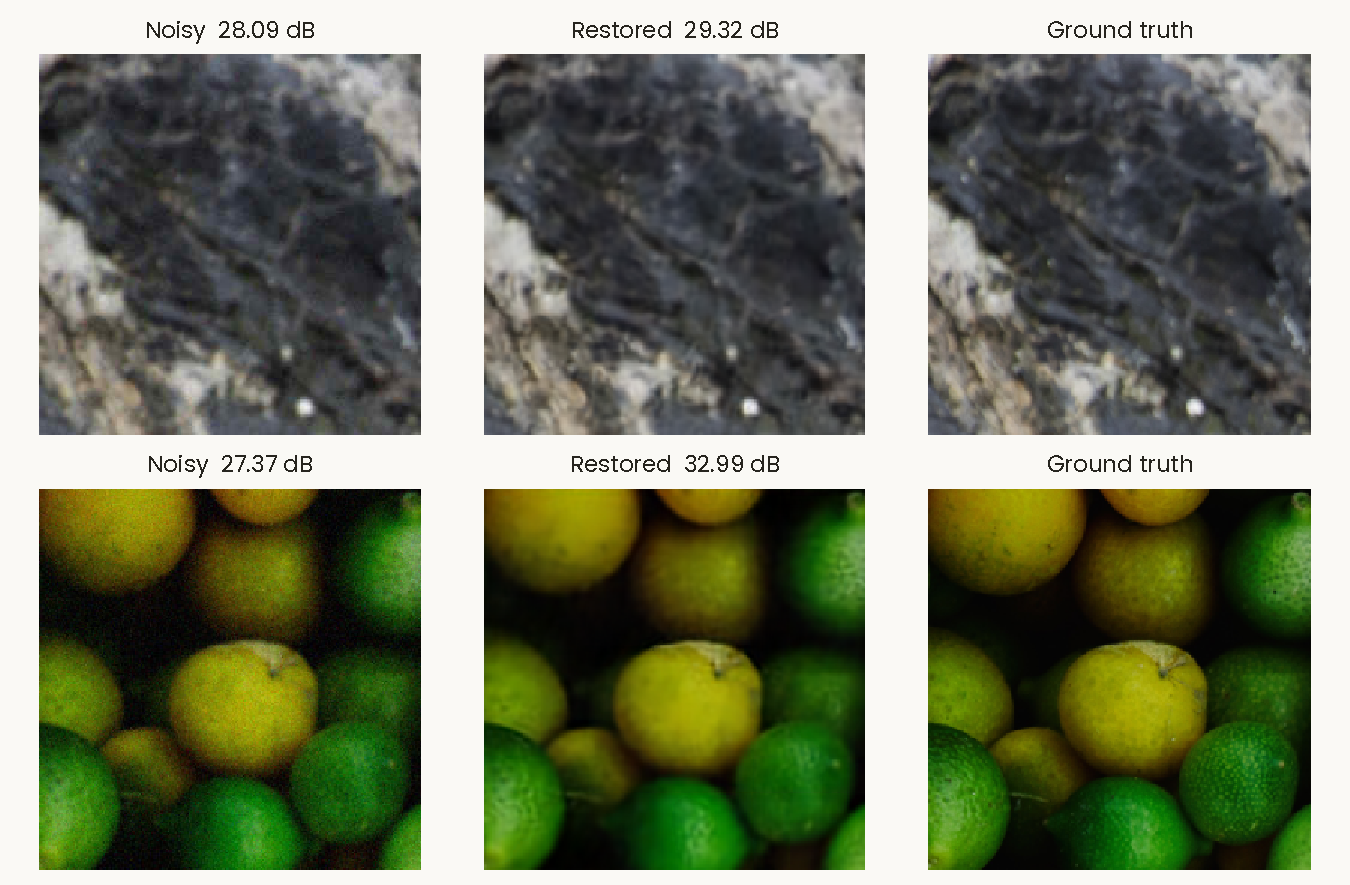
\includegraphics[width=0.85\linewidth]{qualitative_fcsg.pdf}
		\caption{\fcsg{}}
	\end{subfigure}\\[1ex]
	\begin{subfigure}{\linewidth}
		\centering
		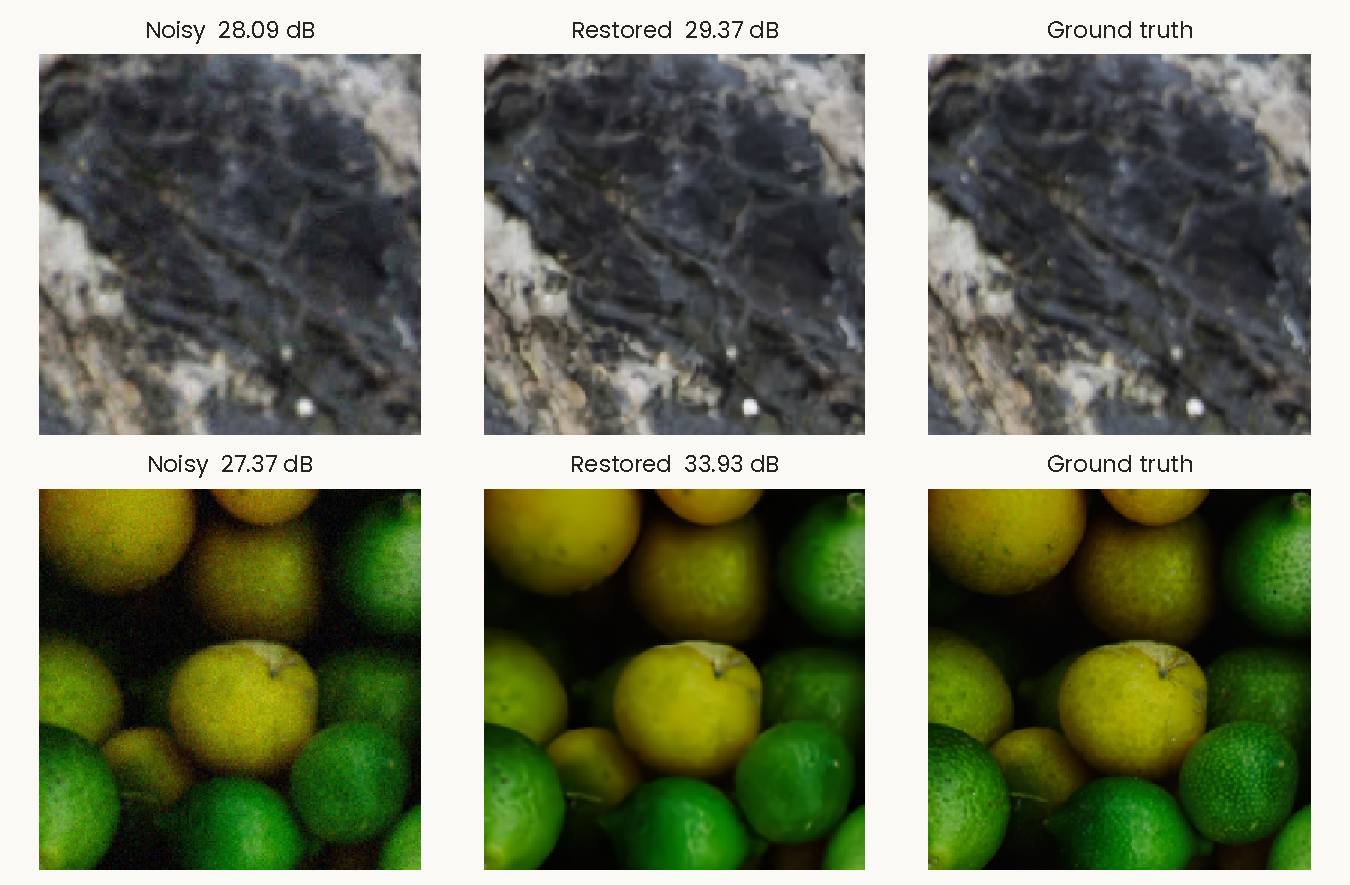
\includegraphics[width=0.85\linewidth]{qualitative_blind.pdf}
		\caption{FFDNet, blind}
	\end{subfigure}
	\caption{Degraded input, restoration and clean target on validation images
	0801 and 0802. The panels show the top-left $320\times320$ region. PSNR is
	for the whole image.}
	\label{fig:qual}
\end{figure}

\section{Computational cost}\label{sec:cost}

Table~\ref{tab:latency} gives the median FP32 forward latency at batch 1 on a
Tesla T4, measured after warm-up.

\begin{table}[htbp]
	\centering
	\caption{Median forward latency (ms) and peak inference memory at $256^2$ (Tesla T4, FP32).}
	\label{tab:latency}
	\small
	\begin{tabular}{@{}lrrrr@{}}
		\toprule
		Method & $128^2$ & $256^2$ & $512^2$ & Peak MB \\
		\midrule
		\fcsg{}          & 5.10 & 19.40 & 75.59 & 51.3 \\
		DnCNN            & 4.22 & 18.04 & 72.47 & 37.8 \\
		FFDNet, blind    & 1.69 &  6.30 & 24.12 & 20.2 \\
		\bottomrule
	\end{tabular}
\end{table}

\fcsg{} needs an eighth of DnCNN's FLOPs and a third of FFDNet's, and it is
still the slowest model at every size, with the highest memory use. Training
told the same story, at 5.84 steps per second against 9.41 for DnCNN and
26.67 for FFDNet. We did not profile individual operators, so our
explanation comes from reading the architecture. Each image goes through nine
full expert passes. Memory traffic, not arithmetic, limits the speed of
depthwise convolutions. Many small layers add launch overhead, and the FFTs
add their own cost. FFDNet runs one stack of dense $3\times3$ convolutions,
which GPUs handle very well. On this hardware, the FLOP budget we set at the
start was the wrong stand-in for speed (Figure~\ref{fig:cost}). Tiling does
not cause the quality gap. Moving from 256 to 512 pixel tiles changes \fcsg{}
by only 0.013\dB{} on a ten-image subset.

\begin{figure}[htbp]
	\centering
	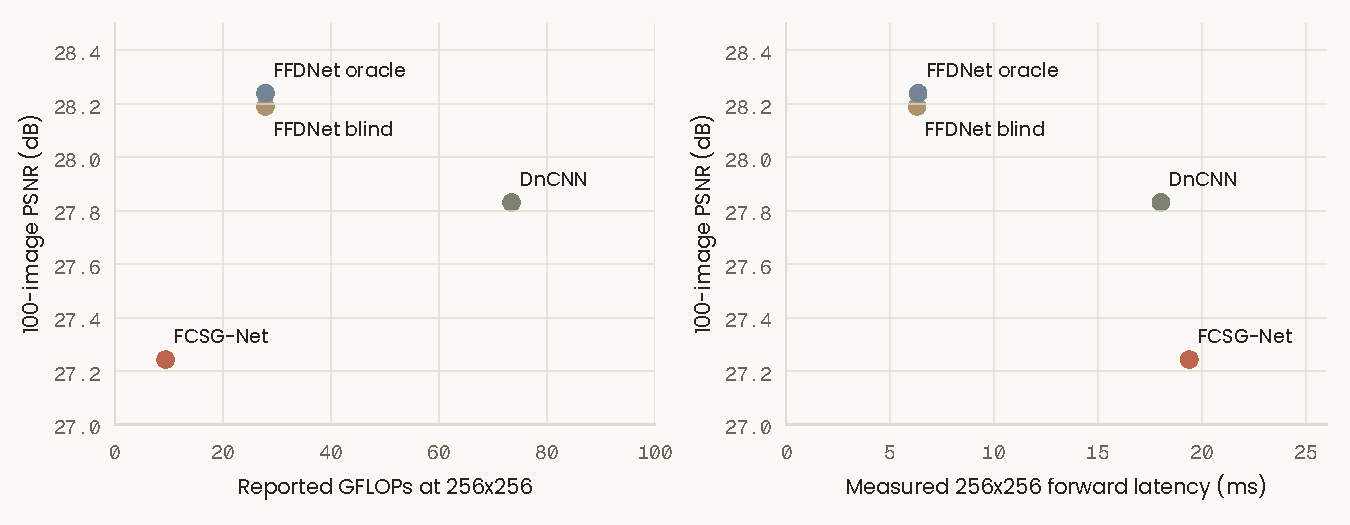
\includegraphics[width=0.95\linewidth]{compute_latency.pdf}
	\caption{Validation PSNR against reported GFLOPs (left) and against
	measured $256\times256$ latency (right).}
	\label{fig:cost}
\end{figure}

\section{Routing analysis}\label{sec:routing}

We studied the final \fcsg{} checkpoint on ten validation images, each
degraded with eight seeds. That gives 80 samples from ten independent images.

\paragraph{Where the gate routes.} The dense routing probabilities end up
close to uniform, with a mean entropy of 1.09 to 1.10 nats per band against a
maximum of 1.10. Taken alone, that suggests the gate learned nothing. The
top-2 selection says otherwise. In the high band the gate picks the
$3\times3$ expert at 99.98\% of pixels, and the larger experts share the
second slot depending on location. The maps follow image structure
(Figure~\ref{fig:routing-map}). Top-2 selection flips when two logits swap
rank, so near-uniform probabilities can still produce a sharp, consistent
choice.

\begin{figure}[htbp]
	\centering
	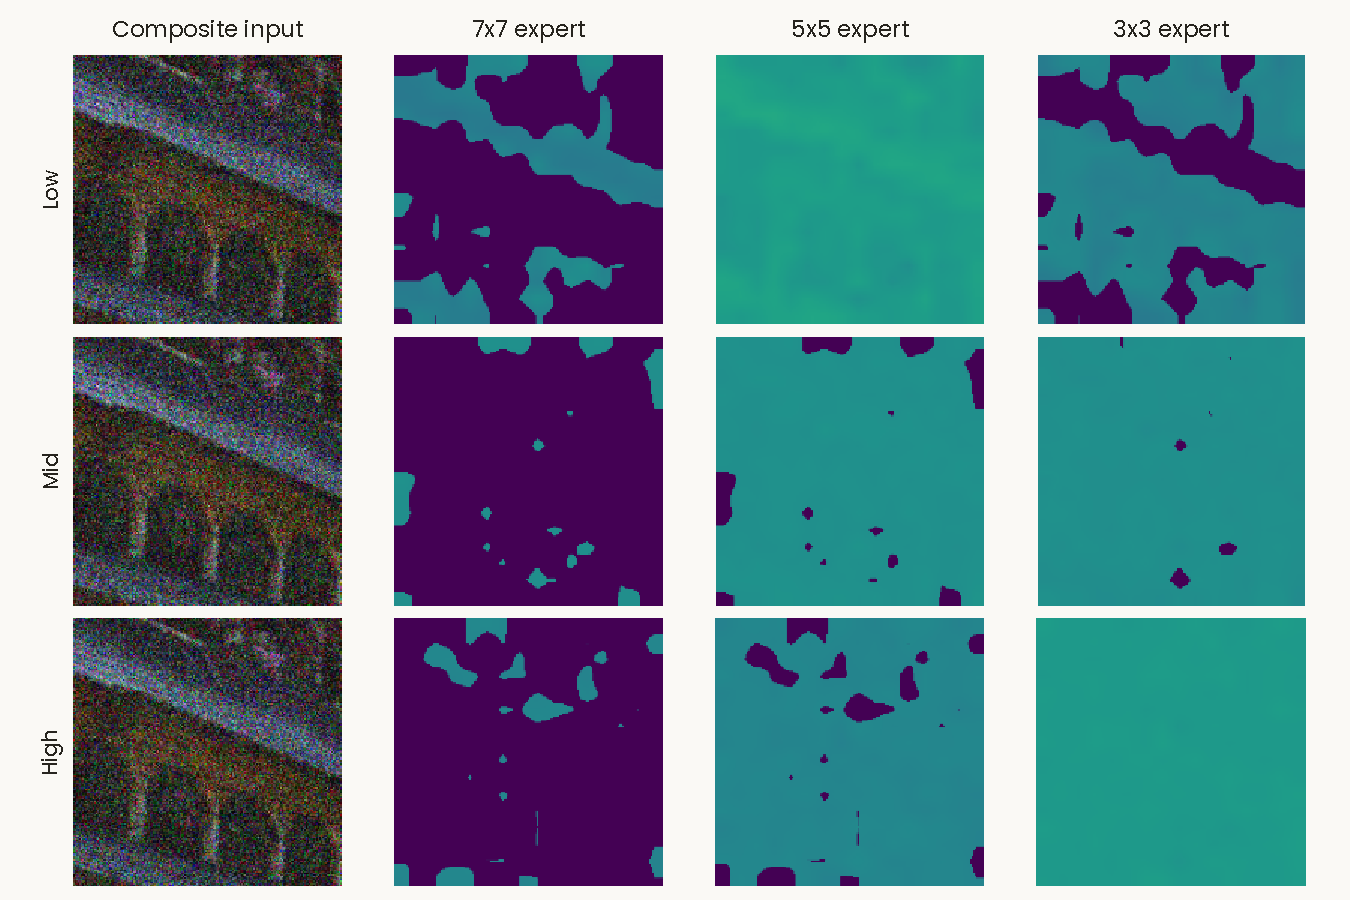
\includegraphics[width=0.9\linewidth]{routing_0834.pdf}
	\caption{Expert weights for validation image 0834. Rows show the low, mid
	and high band. Columns show the degraded crop and the weights of the
	$7\times7$, $5\times5$ and $3\times3$ experts.}
	\label{fig:routing-map}
\end{figure}

\paragraph{Routing and the degradation.} After subtracting each image's
mean, the high-band $3\times3$ weight correlates at $r=+0.81$ with the noise
level. The low-band $5\times5$ weight correlates at $+0.80$ and the low-band
$7\times7$ weight at $-0.73$. More noise moves weight toward smaller kernels.
All six of the strongest correlations involve noise. The strongest with blur
is $+0.42$ and the strongest with JPEG quality is $-0.39$. These results are
exploratory. They come from ten images and 36 correlations with no
multiple-comparison correction, and the four parameters move together. They
show a consistent response, not a causal one.

\paragraph{Does the model need the gate?} We kept the trained weights and
overrode the gate at inference. Table~\ref{tab:interventions} gives the
result.

\begin{table}[htbp]
	\centering
	\caption{PSNR change when we override the trained gate at inference (10 images).}
	\label{tab:interventions}
	\small
	\begin{tabular}{@{}lrr@{}}
		\toprule
		Intervention & Mean $\Delta$PSNR & Min / max \\
		\midrule
		Equal weights on the selected pair     & $-0.040$\dB & $-0.137$ / $+0.028$ \\
		Uniform weights over all three experts & $-0.372$\dB & $-0.986$ / $+0.163$ \\
		\bottomrule
	\end{tabular}
\end{table}

Flattening the weights inside the chosen pair barely matters. Dropping the
choice itself costs 0.37\dB{} on average and nearly 1\dB{} on one image. The
trained network cares far more about \emph{which} experts are combined than
about how they are weighted. So the gate does real work in this model.
Whether a model trained without a gate would do worse is a separate question
that needs a matched training ablation, which we leave to future work.

\section{Discussion}\label{sec:discussion}

The routing works in the sense we set out to test. It varies across the
image, follows the noise level and matters to the trained model. It does not
make the model competitive. With under 100,000 parameters, \fcsg{} trails
baselines six to nine times its size by 0.6 to 1.0\dB{}, most likely for lack
of capacity, and it is no faster on a GPU. Frequency-band routing is a cheap
way to make a small model's behaviour visible. Within our budget, it does not
on its own make the model better or faster.
